\documentclass[11pt]{article}
\usepackage{amssymb}
\usepackage{amsmath,amscd,amsthm}
\usepackage[utf8]{inputenc}
\usepackage[english,russian]{babel}
\usepackage{pscyr}
\usepackage{hyperref}
\usepackage{indentfirst}
\usepackage{slashed}
%\usepackage{letltxmacro}
\usepackage{mathtools}
\usepackage{ulem}
\usepackage{xcolor}
%\thispagestyle{empty}
\usepackage{graphicx}
\graphicspath{ {images/} }
\usepackage{multirow}
\usepackage{amsmath}
\usepackage{comment}
%\usepackage{times}
\usepackage{tikz}
\usepackage[all]{xy}
\xyoption{tips}
\SelectTips{lu}{10}
 \usetikzlibrary{matrix,calc,arrows,shapes,snakes,positioning}

\def\be{\numberwithin{equation}{section}\begin{eqnarray}}
\def\ee{\end{eqnarray}}
\def\trademark{{\hbox{\tiny TM}}}
\def\dim{\textmd{dim} \hskip 3 pt}
\def\p{\partial}
\def\R{\Rightarrow}
\def\ph{\varphi}
\newtheorem{thm}{Theorem}[section]
\newtheorem{cor}[thm]{Corollary}
\newtheorem{lem}[thm]{Lemma}
\theoremstyle{remark}
\newtheorem{rem}[thm]{Remark}
\theoremstyle{definition}
\newtheorem{Def}[thm]{Definition}

\setcounter{section}{-1}

\newcommand{\que}[1]{\footnote{\textcolor[rgb]{0.38,0.69,0.82}{#1}}}

\renewcommand\thefootnote{\textcolor[rgb]{0.38,0.69,0.82}{\arabic{footnote}}}


\LetLtxMacro{\oldsqrt}{\sqrt} % makes all sqrts closed
\renewcommand{\sqrt}[1][\ ]{%
  \def\DHLindex{#1}\mathpalette\DHLhksqrt}
\def\DHLhksqrt#1#2{%
  \setbox0=\hbox{$#1\oldsqrt[\DHLindex]{#2\,}$}\dimen0=\ht0
  \advance\dimen0-0.2\ht0
  \setbox2=\hbox{\vrule height\ht0 depth -\dimen0}%
  {\box0\lower0.71pt\box2}}

%$\sqrt[a]{b} \quad \oldsqrt[a]{b}$

%%%%%%%%%%%%%%%%%%%%%%%%%%%%%%%%%%%%%%%%%%%%%%%%%%%%%%%%%%%%%%%%%%%%%%%%
%%%%%%%%%               SPACE FILLING SETTINGS               %%%%%%%%%%%
%%%%%%%%%%%%%%%%%%%%%%%%%%%%%%%%%%%%%%%%%%%%%%%%%%%%%%%%%%%%%%%%%%%%%%%%
\textheight 23.5cm \textwidth 16.3cm
%\voffset=-1.2in
\voffset=-0.8in
%\voffset= - 1.85in
\hoffset= - 1.0in         % switch off for draft style
\multlinegap=1.0in
%%%%%%%%%%%%%%%%%%%%%%%%%%%%%%%%%%%%%%%%%%%%%%%%%%%%%%%%%%%%%%%%%%%%%%%%

\begin{document}

\baselineskip14pt
\bigskip


\tableofcontents
\bigskip
\bigskip

%======================================================

А.С. нам рассказывает вещи, которые не должны быть утеряны. Каждый раз он рассказывает, каковой (по-видимому) на самом деле должна быть парадигма. Здесь будет записываться <<передний фронт разработки>>, как в программировании. (Таким образом, это не конспект нашего семинара.)

Пожалуйста, \textbf{вносите изменения} в этот файл, \textbf{дополняйте} его. Пусть он станет вашим рабочим столом. Нет никакого другого способа что-то понять, чем попытаться изложить это листу бумаги/соседу/уточке в ванной. Но у изложения листу бумаги есть два дополнительных бонуса:
\begin{itemize}
  \item не пропадёт ваш скорбный труд и дум высокое стремленье
  \item возможность конструктивного фидбека от $n$ слушателей семинара
\end{itemize}

\section{Как вносить изменения в файл}

Если вы обнаруживаете, что чего-то не понимаете --- предлагаю задать вопрос сноской. Делается это с помощью синтаксиса $\backslash \text{que} \{ \text{почему?} \}$. Пример\que{почему?} заданного таким образом вопроса.

Если вы обнаруживаете, что что-то понимаете --- просто берёте и редактируете текст.

Если у вас не компилится этот tex-файл --- закомментируйте строку $\backslash\text{usepackage}\{ \text{pscyr} \}$ и попробуйте снова; пакет pscyr, содержащий красивые кириллические шрифты, не все себе устанавливали.

В качестве системы контроля версий мы будем использовать GitHub (сейчас это фактически стандарт индустрии).

\subsection{Зачем нужна система контроля версий?}

Зачем Волга впадает в Каспийское море, а хлоропласты --- зелёные?

GitHub основан на Git. Их плюсы:

\begin{itemize}

\item У Git не бывает ошибок при синхронизации, в отличие от многих других систем совместной разработки (например, shared Dropbox folder творит ерунду, когда трое или больше человек одновременно работают над файлом)

\item Git сохраняет абсолютно все версии отслеживаемых файлов. Каждый раз, когда вы делаете коммит, вы сохраняете в специальной скрытой папке снимок состояния вашего проекта, который можете позже восстановить или с которым можно сравнить текущее состояние.

\item Удобно, что проект публичен и имеет короткий, простой и понятный, милый нашему сердцу веб-адрес ---
\href{https://github.com/m-theory/book}{\textcolor[rgb]{0.38,0.69,0.82}{github.com/m-theory/book}}.

\end{itemize}

Минус у Git/GitHub только один --- относительная сложность освоения. Но вас никакие сложности не коснутся, потому что ниже по пунктам расписано, что и как делать.

\subsection{Linux-мануал}

\subsubsection{При первом использовании}


Сначала необходимо установить git. Для этого, как знает каждый Linux-юзер, нужно запустить Terminal/Konsole и установить соответствующий пакет. В Ubuntu 14.04 это делается командой \begin{verbatim}sudo apt-get install git\end{verbatim}
В других дистрибутивах эта команда может выглядеть по-другому, но каждый Linux-пользователь знает, как она выглядит для его дистрибутива.


Далее необходимо сделать клон на своём локальном компьютере текущей версии репозитория m-theory: \begin{verbatim}git clone https://github.com/m-theory/book.git\end{verbatim}
Такой клон называется локальным репозиторием. \textit{(В Git/GitHub у каждого из проектов, над которым работает разработчик, есть по репозиторию; именно в репозиториях хранятся файлы.)}

В результате выполнения такой команды репозиторий будет склонирован в папку $\sim$/book. Зайдём же в неё.  \begin{verbatim}cd book\end{verbatim}

Полюбуемся на файлы в ней:\begin{verbatim}ls\end{verbatim}

Попробуем внести изменение в tex-файл. Откроем его texmaker'ом (или вашим любимым текстовым редактором --- vim, nano, kate, gedit, emacs):\begin{verbatim}texmaker paradigm.tex\end{verbatim}

Внесли изменения. Внесли? Отлично.

Давайте полюбуемся на внесённые изменения:

\begin{verbatim}git diff paradigm.tex\end{verbatim}

Более чем наглядно, не правда ли? \textit{(Выйти из процесса git:diff можно нажатием клавиши q.)}

\begin{comment}
Далее необходимо добавить в индекс текущую версию изменившихся файлов. Если просто добавлять в индекс все файлы в репозитории командой git add ., то на диске такого участника будет сохраняться не только 654 версии файлов paradigm.tex и paradigm.pdf, но и 654 версии бесполезных служебных файлов, возникающих во время процедуры PDF\LaTeX. С другой стороны, явно каждый раз прописывать файлы, которые мы хотим индексировать (это две команды git add paradigm.tex, git add paradigm.pdf), довольно утомительно. Чтобы не делать этого, создаём файл .gitignore:
\begin{verbatim}touch .gitignore\end{verbatim}

Откроем этот файл любым текстовым редактором, например,
\begin{verbatim}nano .gitignore\end{verbatim}

и пропишем в нём следующие строки:
\begin{verbatim}
*.aux
*.blg
*.log
*.synctex
*.synctex.gz
*.toc
*.bbl
*.nav
*.out
*.snm
\end{verbatim}
Тем самым мы говорим Git, что нужно игнорировать все файлы с этими расширениями. То есть, система контроля версий не будет отслеживать изменения во всех файлах этих типов.
\end{comment}


Далее необходимо пометить интересные нам файлы как отслеживаемые (добавить их под версионный контроль). Если пометить как отслеживаемые все файлы репозитория командой git add . и затем делать коммиты, то на диске такого разработчика будут сохраняться не только 654 версии файлов paradigm.tex и paradigm.pdf, но и 654 версии таких невероятно полезных файлов, как paradigm.aux, paradigm.log, paradigm.blg, paradigm.toc, (я могу долго перечислять), возникающих во время процедуры PDF\LaTeX. Это была бы лишь трата места на жёстком диске. К счастью, в нашем случае мы можем заранее назвать все файлы, которые мы хотим индексировать, так что удобно просто выполнить две команды
\begin{verbatim}git add paradigm.tex\end{verbatim}
\begin{verbatim}git add paradigm.pdf\end{verbatim}

Что это? Зачем это нужно? Здесь уместно ещё раз проговорить, что Git --- это система контроля версий. Командами git add мы создали указатель на текущие версии файлов paradigm.tex и paradigm.pdf. После совершения так называемого коммита в скрытой папке /.git/ будут созданы слепки этих текущих версий. Оттуда Git способен полностью восстановить любую из версий любого из отслеживаемых файлов. Каждый раз, когда вы делаете коммит, вы сохраняете снимок состояния вашего проекта, который можете позже восстановить или с которым можно сравнить текущее состояние.

Пытаемся сделать коммит\begin{verbatim}git commit -m "Внёс небольшие правки; в частности, задал пару вопросов в сносках"\end{verbatim}
но, внезапно, нам выкатывают такую предъяву:

Please tell me who you are.

git config \text{-}\text{-}global user.email "you@example.com"

fatal: unable to auto-detect email address

\bigskip

Действительно, GitHub просит публиковать e-mail'ы тех, кто делает коммиты (=разработчиков). Это необходимо, чтобы, увидев на гитхабе восхитительный проект, заинтересованные лица могли связаться с его авторами. Словом, ничего не поделаешь, придётся послушаться и выполнить команду
\begin{verbatim}git config --global user.email "yourmail@xxx.xxx"\end{verbatim}
и теперь всё получится
\begin{verbatim}git commit -m "Внёс небольшие правки; в частности, задал пару вопросов в сносках"\end{verbatim}

Сообщение, отражающее суть изменения (commit message), надо писать обязательно!

Ура, теперь текущее состояние файлов, с которыми вы работаете, сохранено в репозиторий. Сделан слепок, из которого вы это текущее состояние сможете в любой момент восстановить.

Последнее, что осталось сделать ---
\begin{verbatim}git push\end{verbatim}
Здесь вы <<толкаете>> свой локальный репозиторий на удалённый сервер.
Здесь вас спросят username и password. Ваш юзернейм m-theory, ваш пассворд вы знаете (а если не знаете, спросите у кого-нибудь из нас).


Всё! Файлы с изменениями публично доступны по адресу \href{https://github.com/m-theory/book}{\textcolor[rgb]{0.38,0.69,0.82}{github.com/m-theory/book}}.



\subsubsection{При использованиях последующих}

Работа начинается с

\begin{verbatim}git pull\end{verbatim}
Здесь отличие. git pull <<тянет>> удалённый репозиторий (расположенный по адресу \href{https://github.com/m-theory/book}{\textcolor[rgb]{0.38,0.69,0.82}{github.com/m-theory/book}} --- более точно, по тому адресу, с которого вы в своё время сделали git clone) на локальную машину, при этом локальный репозиторий будет перезаписан. Это необходимо, когда вы не уверены в том, что именно вы внесли последнюю правку в файлы нашего <<официального>> репозитория \href{https://github.com/m-theory/book}{\textcolor[rgb]{0.38,0.69,0.82}{github.com/m-theory/book}} (т.е. необходимо почти всегда).

\begin{verbatim}cd book\end{verbatim}

\begin{verbatim}texmaker paradigm.tex\end{verbatim} (вносим изменения; необязательный шаг --- полюбоваться на них командой git diff paradigm.tex) \textit{(выйти из открывшегося процесса book:git можно нажатием клавиши q)}



\begin{verbatim}git commit -a -m "Внёс небольшие правки; в частности, задал пару вопросов в сносках"\end{verbatim}

Сообщение, отражающее суть изменения (commit message), надо писать обязательно! Директива -a автоматически делает git add для всех файлов, которые уже являются отслеживаемыми.

\footnotesize{}

\textbf{Q}: Зачем git add, зачем снова добавлять файлы в отслеживаемые?

\textbf{A}: git commit создаёт слепок файлов в том состоянии, в котором они были на момент последнего выполнения git add. Так что следует сначала вносить изменения, и лишь затем выполнять git add filename(s) и git commit. К счастью, последние две команды можно объединить в одну (git commit -a).

\normalsize{}

Мы не предполагаем, что в проекте появятся другие значимые файлы, помимо paradigm.tex и paradigm.pdf, что появятся другие файлы, которые следует отслеживать. Если они появятся, то непосредственно перед коммитом необходимо сделать одну или несколько команд вида git add newfile.tex.

Осталось лишь отправить результат наших правок на <<официальный репозиторий>>:

\begin{verbatim}git push\end{verbatim}
Здесь всё то же самое: username m-theory, пароль вы знаете.




\subsection{Windows-мануал}


\subsubsection{При первом использовании}

Заходим на \href{https://github.com/}{\textcolor[rgb]{0.38,0.69,0.82}{github.com}}, листаем вниз, долистываем до кнопки <<Download GitHub for Windows>>. Устанавливаем.

После установки запустится замечательный графический интерфейс. Он скажет <<Welcome>> и предложит залогиниться. Username наш m-theory, пароль вы знаете (а если не знаете, то спросите у кого-нибудь из нас).

На шаге <<Configure>> вам просто нужно нажать Continue.

На шаге поиска локальных репозиториев нажать Skip. Всё, вас отпустило, и вам пишут <<Get started by adding a repository>>.

В левом верхнем углу вашего внимания добивается пульсирующая кнопка <<+>>. Жмём на неё, выбираем вкладку Clone, нажимаем на book. Clone book.

Отлично! Вы в раю. Ваши файлы находятся, скорее всего, в папке /Документы/GitHub/book/. Вы можете изменять их там как хотите и копировать в эту папку что хотите.

Как только содержимое этой папки малейшим образом изменится, в приложении GitHub (надеюсь, вы его ещё не закрыли?..) появится оповещение <<Uncommitted changes>>. Нажимаем на Show. Пишем что-нибудь в <<Message>> и <<Description>>, делаем коммит. После чего замечаем, что справа от кнопки Sync есть $\uparrow$1, что как бы намекает нам залить изменения с локальной машины на <<официальный>> репозиторий \href{https://github.com/m-theory/book}{\textcolor[rgb]{0.38,0.69,0.82}{github.com/m-theory/book}}.

Вы восхитительны! Ваши изменения вписаны золотыми буквами в историю \href{https://github.com/m-theory/book}{\textcolor[rgb]{0.38,0.69,0.82}{github.com/m-theory/book}}. Просто пройдите туда и взгляните.


\subsubsection{При использованиях последующих}

Если в публичном репозитории \href{https://github.com/m-theory/book}{\textcolor[rgb]{0.38,0.69,0.82}{github.com/m-theory/book}} кипела работа, пока вы наслаждались жизнью, то у кнопки Sync в правом верхнем углу будет ненавязчиво привлекать к себе внимание циферка (количество коммитов, сделанных другими людьми). Кнопку Sync в таком случае неплохо б нажать, чтобы загрузить на свой компьютер результаты работы других людей (самое свежее состояние проекта).

Важный момент, о котором осталось сказать. Если вы компилируете этот tex-файл в той же папке (/Документы/GitHub/book/), у вас постоянно обновляются разные автоматически генерируемые файлы (обычно это paradigm.aux, paradigm.log, paradigm.blg, paradigm.toc и paradigm.synctex.gz). Как уже было сказано, Git сохраняет слепок каждого из файлов, за которым он <<следит>>. Эти слепки хороши в том смысле, что по ним можно восстановить каждую из версий файлов, но в случае .aux, .log, ... файлов они просто засоряют ваш диск. Можно приказать Git не делать слепки этих файлов.
Для этого нажимаем на (символизирующую настройки) шестерёнку, выбираем <<Repository settings>>. Выбираем Add a default .gitignore file, НО НЕ нажимаем Update. В этот файл необходимо добавить следующие строки:

\begin{verbatim}
*.aux
*.blg
*.log
*.synctex
*.synctex.gz
*.toc
*.bbl
*.nav
*.out
*.snm
\end{verbatim}

Проследите за тем, чтобы эти строки не начинались со знака \# (иначе Git их проигнорирует как комментарий). Теперь нажимаем Update. В чём смысл? В том, что Git теперь будет игнорировать изменения в файлах с такими расширениями, т.е. не будет записывать их слепки на жёсткий диск. Чего и требовалось добиться.

\newpage

\section{$A_{\infty}$-структуры, $\Delta_{BV}$-оператор, поливекторные поля}

\subsection{Наша задача --- понять, что вместо вопроса}

(Пока что наша задача --- великолепно переписать этот огрызок.)

Есть нечётные \que{Что это такое?} векторные поля $v_{\text{н}}$: $$v_{\text{н}} \in \oplus_k V^{\otimes k} \to V.$$

И главное уравнение $A_{\infty}$-структуры \que{Что это такое?} имеет вид: $v_{\text{н}}^2 = 0.$ Или $\{v,v\}_G = 0.$

Но неправильно говорить просто об этом уравнении. Нужно ещё сфакторизовать по соотношению эквивалентности $v\sim v + \{v,w\}$ --- автоморфизмам этого векторного пространства.

$$v = v_0 + Pol, \hskip 20 pt Pol \ll v_0.$$ Получится уравнение $\{ v_0, Pol \} + \{ Pol, Pol \} = 0.$

Далее, можно сказать, что $Pol = P_0 + \omega$. Т.е. $v = v_0 + P_0 + \omega$. Именно $\omega$, этот чёртов третий член, даёт нам когомологии. Первые же два члена этого разложения определяют мир, который рассматривается.

Стоит отметить, что $v_0: V^{\otimes 2} \to V$ --- обычное умножение. Поэтому его обычно обозначают $m_2$.

Если мы работаем с кольцом $\mathbb{C}[x] \otimes \mathbb{C}[\lambda, \theta] / (\lambda \gamma \lambda)$ (пространственных переменных $x$ 10, чётных полей $\lambda$ 16, нечётных полей $\theta$ тоже 16), а в качестве $P_0$ мы берём $\lambda^{\alpha} \frac{\partial}{\partial \theta^{\alpha}}$, то получится $\mathcal{N} = 1$ $D=10$ SYM \que{интересно, какая из пяти?..}. Низкоэнергетическое приближение --- $D=10$ супергравитация.

Получается такой коммутативный квадрат:

%$$\xymatrix{ ? \ar@{.>}[r] \ar@{.>}[d] & \text{nearly comm.limit\que{что это?}} \ar[d] \\ \hbar\Delta_{BV} Pol+ \{Pol, Pol\} = 0 \ar[r] & \{Pol, Pol\} = 0}$$

\begin{center}
\begin{tikzpicture}[>=stealth',shorten >=1pt,auto,node distance=3cm,
  thick,back line/.style={densely dotted},
cross line/.style={preaction={draw=white, -,
line width=6pt}},main node/.style={circle,fill=blue!20,draw,font=\sffamily\Large\bfseries}]

\matrix (m) [matrix of math nodes,
row sep=3em, column sep=3em,
text height=1.5ex,
text depth=0.25ex]{
? &  & \text{nearly comm.limit} \\
 & & \\
\hbar\Delta_{BV} Pol+ \{Pol, Pol\} = 0 &  & \{Pol, Pol\} = 0 \\
};

% Сноску "что это?" из коммутативной диаграммы никак не поставишь --- я пытался. Поэтому так.

\path[->]
(m-1-1) edge [back line] (m-3-1)
(m-1-1) edge [back line] (m-1-3)
(m-3-1) edge (m-3-3)
(m-1-3) edge (m-3-3);
\end{tikzpicture}

\end{center}

И наша задача --- понять, что вместо вопроса.

\subsection{Задача матричной факторизации}

Точки на нашем пространстве модулей могут подъезжать к границе, и нужно предложить какое-то граничное условие. Граница является браной.

Сама по себе задача матричной факторизации давно известна в теории особенностей и сводится к элементарному утверждению. Именно, нужно решить матричное уравнение на $N$ вида $W = N^2$. $W(x)$ --- суперпотенциал, $N$ --- матрица, которую необходимо найти.\que{Тема матриц не раскрыта} Высший смысл происходящего формулируется так: триангулированные категории особенностей слоёв отображения $W$ эквивалентны категориям В-бран.


\begin{comment}
\footnotesize{}

Общеобразовательный кусок про деформации комплексных структур

$$Q_{\tau} = Q + \tau V_1 + \tau^2 V_2, \bar \p_{\tau} = \bar\p + \tau \mu_1 \p + \tau^2 \mu_2 \p + ...$$

Надо изучать комплексные структуры по модулю диффеоморфизмов. Оказывается, уравнение Кодаиры $$(\bar\p + \mu(\tau) \p)^2 =0$$ можно обобщить. А именно, можно деформировать не только дифференциал $\bar\p$, но и вообще всё что угодно.

В топологической квантовой механике имеем уравнение $$H = \{Q(\tau), G\}.$$

\normalsize{}

\end{comment}


\section{Новый взгляд на геометрию}
\subsection{Собственно взгляд}

Классическая геометрия является вырождением геометрии Полякова.

\begin{center}


\begin{comment}
\begin{tikzpicture}[
back line/.style={densely dotted},
cross line/.style={preaction={draw=white, -,
line width=6pt}}]
\end{comment}

\begin{tikzpicture}[>=stealth',shorten >=1pt,auto,node distance=3cm,
  thick,back line/.style={densely dotted},
cross line/.style={preaction={draw=white, -,
line width=6pt}},main node/.style={circle,fill=blue!20,draw,font=\sffamily\Large\bfseries}]


%\shade[shading=radial, inner color=blue]
%(0,0) rectangle (2,1);

 % \matrix[nodes={fill=blue!20},
%       row sep=7em,column sep=3em,text height=1.5ex,
% text depth=0.25ex]
%{
%    \node[ellipse] {\text{яяя}}; \\};

\matrix (m) [matrix of math nodes,
row sep=3em, column sep=3em,
text height=1.5ex,
text depth=0.25ex]{
& \text{Геометрия} & & \text{Физика} \\
\text{гладкие мн-я} & & \text{классическая} \\
& \text{алг. геом.} & & \text{квант. мех.} \\
 & & & \textmd{некомм. геом.} \\
  & \text{Поляков} & &  \\
};

\draw (m-2-1) edge [back line] node {\tiny{\text{Риччи-плоск.;\hskip 20 pt инстантоны}}} (m-2-3)
(m-2-3) edge [back line] node {\tiny{\text{идеи Фейнмана}}} (m-3-4)
(m-3-2) edge [back line] node {\tiny{\text{некомм. алгебра}}} (m-3-4);
%(m-3-2) edge (m-4-1)
%(m-3-4) edge (m-4-3)
%(m-2-1) edge [back line] (m-4-1)

%(m-2-3) edge [back line] (m-4-3)
\path[->]
(m-1-2) edge (m-2-1)
(m-1-4) edge (m-3-4)
(m-3-4) edge (m-4-4)
(m-1-2) edge [cross line] (m-3-2)
(m-2-3) edge [cross line] (m-5-2)
(m-4-4) edge (m-5-2)
(m-1-4) edge (m-2-3);
%(m-4-1) edge (m-4-3)
\end{tikzpicture}

\end{center}



Есть две точки зрения на то, что изучает геометрия:

\begin{itemize}
  \item пространство
  \item пространство и какая-нибудь геометрическая структура на нём
\end{itemize}

Согласно Полякову, (гомотопическая) конформная теория --- это и есть пространство + геометрия на нём.

\subsection{Напоминание о том, что такое конформная теория поля}

Конформные теории поля --- теории поля, инвариантные относительно конформных преобразований метрики. В них есть <<основной объект>> $I$, зависящий от поверхности $\Sigma$ (вид поверхности зависит от того, открытая или замкнутая струна, а также от количества наблюдаемых $V_1$, ..., $V_n$ в рассматриваемом корреляторе). Метрик, сфакторизованных по соотношению эквивалентности <<конформно связанные метрики эквивалентны>>, столько же, сколько комплексных структур, поэтому основной объект $I$ зависит также от комплексной структуры (т.е. от дифференциала Бельтрами $\mu$, который параметризует модули комплексных структур на $\Sigma$). Комплексные структуры, очевидно, надо изучать по модулю диффеоморфизмов. Физический смысл нижеследующей картинки вот каков: для того, чтобы вычислить коррелятор операторов $V_1$, ..., $V_n$, нужно вырезать малые диски вокруг точек worldsheet'а и вычислять инварианты Громова---Виттена, являющиеся подсчётом композиций кобордизмов комплексно одномерных многообразий\que{я правильно понимаю, что основной объект $I(\Sigma, V_1, ..., V_n)$ и соответствующий ему инвариант Громова---Виттена --- это одно и то же?}.

\begin{center}
\begin{tikzpicture}

%\fill[cyan!10] (-0.1,0.4) arc (-45:45:1cm and 1.55cm) arc (-95:40:0.166cm and 0.5cm) arc (-175:-5:2.0cm and 0.53cm) arc (140:275:0.166cm and 0.5cm) arc (135:225:1cm and 1.55cm) arc (85:220:0.166cm and 0.5cm) arc (5:175:2.0cm and 0.53cm) arc (-40:95:0.166cm and 0.5cm);

\fill[cyan!10] (4,0) rectangle (0,3);

\fill[cyan!10] (0.11,3.4) arc (-175:-5:1.9cm and 0.6cm) -- (3.89,2.45) -- (0.11,2.45) -- cycle;
\fill[cyan!10] (3.89,-0.4) arc (5:175:1.9cm and 0.6cm) -- (0.11,0.55) -- (3.89,0.55) -- cycle;

%	\draw[dashed,color=gray] (0,0) arc (-90:90:0.5 and 1.5);% right half of the left ellipse
%	\draw[semithick] (0,0) -- (4,1);% bottom line
%	\draw[semithick] (0,3) -- (4,2);% top line
%	\draw[semithick] (0,0) arc (270:90:0.5 and 1.5);% left half of the left ellipse
	\draw[thick,fill=white] (4,3) ellipse (0.166 and 0.5);% right top ellipse
	\draw[thick,fill=white] (0,3) ellipse (0.166 and 0.5);% left top ellipse
	\draw[thick,fill=white] (4,0) ellipse (0.166 and 0.5);% right bottom ellipse
	\draw[thick,fill=white] (0,0) ellipse (0.166 and 0.5);% left bottom ellipse
\draw[thick,fill=white] (-0.1,0.4) arc (-45:45:1cm and 1.55cm); % left arc
\draw[thick,fill=white] (3.89,-0.4) arc (5:175:1.9cm and 0.6cm); % bottom arc
\draw[thick,fill=white] (4.1,2.6) arc (135:225:1cm and 1.55cm); % right arc
\draw[thick,fill=white] (0.11,3.4) arc (-175:-5:1.9cm and 0.6cm); % top arc

  \draw (-0.5,0) node {\footnotesize $...$};
  \draw (-0.5,3) node {\footnotesize $V_1$};
  \draw (4.5,0) node {\footnotesize $V_n$};
  \draw (4.5,3) node {\footnotesize $V_2$};

  \draw (0.75,1.5) node {\footnotesize $\Sigma_1$};
    \draw (2.75,1.5) node {\footnotesize $\Sigma_2$};

\draw[dashed,thick,color=gray] (1.5,1.5) ellipse (0.1cm and 1.37cm);


%\filldraw[fill=cyan, draw=blue] (6,6) -- (12mm,0mm) arc (0:30:12mm) -- (6,6);
\end{tikzpicture}
\end{center}



Т.е. вот где основной объект принимает значения: $$I (\Sigma, \mu) \in V_1 \otimes ... \otimes V_n \otimes \Big( \mu(\Sigma)/\text{diff} \Big)$$

и при этом есть единственная аксиома: что если эту поверхность разрезать, то
$$I(\Sigma, \mu) = I(\Sigma_1, \mu) \circ I(\Sigma_2, \mu).$$

Тензор энергии-импульса же можно вытащить из такой теории вариацией основного объекта по дифференциалу Бельтрами:

$$T = \frac{\delta I(\Sigma, \mu)}{\delta \mu}$$



Польчинский пишет действие, которое мы назовём действием старой струнной геометрии:

$$S = \int g_{\mu\nu} (x) dx^{\mu} \ast dx^{\nu} + B_{\mu\nu}(x) dx^{\mu} \wedge dx^{\nu},$$

второй член --- поле Калба---Рамона, 2-форма на таргете. Действие новой же струнной геометрии таково:


\be  S = \int\limits_{\Sigma} \Bigg( P_i \bar \partial X^i + \bar P_{\bar i} \partial \bar X^{\bar i} + \tikz[baseline]{\draw[dashed,thick,color=gray] (-4.3,-0.25) rectangle (4.3,0.55);
            \node[anchor=base] (t1)
            {$g^{i \bar j} (x, \bar x) P_i P_{\bar j} +\mu^i_{\bar j} P_i \bar \partial \bar X^{\bar j} + \mu_j^{\bar i} P_{\bar i} \partial X^j +  b_{i \bar j} \partial X^i \bar\partial \bar X^{\bar j}$};}  \Bigg). \ee

С помощью комплексной структуры $J$ можно переходить от старой геометрии к новой и, почти всегда, наоборот:

\be (G, B) \xleftrightarrow{J} (\tikz[baseline]{
            \node[fill=purple!20,anchor=base] (t1)
            {$g$};}, \tikz[baseline]{
            \node[fill=orange!20,anchor=base] (t1)
            {$\mu$};}, \tikz[baseline]{
            \node[fill=green!20,anchor=base] (t1)
            {$\bar \mu$};}, \tikz[baseline]{
            \node[fill=cyan!20,anchor=base] (t1)
            {$b$};}).
            \ee


Поговорим про теорию $$S = \int\limits_{\Sigma} P_i \bar \partial X^i.$$ В ней есть поля размерности $(\bullet, 0)$. Это, конечно, функции $f(x) \in (0,0)$, но также и $(\operatorname{Vect} \oplus \Omega) \in (1,0)$ --- алгебра векторных полей, расширенная своими представлениями. Такие элементы образуют алгебру Ли, назовём её $L$.

Новая геометрия лежит в $L \otimes \bar L$. Именно, произведём следующее несложное вычисление:

$$(V \oplus \Omega^1) \otimes (\bar V \oplus \bar \Omega^1) = $$

\begin{equation*}
= \tikz[baseline]{
            \node[fill=purple!20,anchor=base] (t1)
            {$V \otimes \bar V$};}  \oplus \tikz[baseline]{
            \node[fill=orange!20,anchor=base] (t1)
            {$V \otimes \bar \Omega^1$};} \oplus \tikz[baseline]{
            \node[fill=green!20,anchor=base] (t1)
            {$\Omega^1 \otimes \bar V$};} \oplus \tikz[baseline]{
            \node[fill=cyan!20,anchor=base] (t1)
            {$\Omega^1 \otimes \bar \Omega^1$};}.
\end{equation*}

Как уже стало понятно из боевой раскраски, $g \in V \otimes \bar V$, $\mu \in V \otimes \bar \Omega^1$, $\bar \mu \in \Omega^1 \otimes \bar V$, $b \in \Omega^1 \otimes \bar \Omega^1$.

Новая геометрия <<чуть>> больше старой:

\begin{center}
\begin{tikzpicture}


	\filldraw[fill=blue!70!white, thick] (0,1) ellipse (1cm and 0.2cm); % top ellipse
	\filldraw[fill=orange!70!white, thick] (0,0) ellipse (1.4cm and 0.28cm); % bottom ellipse

\draw[dashed,thick,color=gray] (0,0) ellipse (1cm and 0.2cm); % bottom ellipse

\draw[dashed,thick,color=gray] (1.0,1) -- (1.0,0);
\draw[dashed,thick,color=gray] (-1.0,1) -- (-1.0,0);

\begin{scope}[decoration={amplitude=.4mm,
        segment length=2mm,post length=1mm}]

      \draw[decorate,orange,thick] (1.45,0) -- ++(5:3);
      \draw[decorate,blue,thick] (1.05,1) -- ++(5:4);
    \end{scope}

      \draw (1.45,0) ++(5:3) node[right] {\footnotesize new geometry};
  \draw (1.05,1) ++(5:4) node[right] {\footnotesize old geometry};

\end{tikzpicture}
\end{center}

Например, в старой геометрии годилась только Риччи-плоская метрика.

Новая геометрия существует на 0-мерных схемах. (А 0-мерные схемы --- это по разным причинам хорошо.)



\footnotesize{}

Говоря <<схема>>, мы, в первую очередь, держим в уме следующий пример:

$$\mathbb{C}[x_1, ..., x_n] / I_{F(x)}.$$

Посредством резольвенты Кошуля это эквивалентно $\mathbb{C}[x_1, ..., x_n, \theta]$ с дифференциалом $Q = F \frac{\partial}{\partial \theta}.$


\normalsize{}


Пространство является гомологическим многообразием с гомологическим векторным полем. (Гомологическое векторное поле --- такое векторное поле $Q = v^i (x) \frac{\partial}{\partial x^i}$, что $Q^2 = 0$.) Для вещественно двумерного многообразия с комплексной структурой условие гомологичности векторного поля означает интегрируемость структуры. Деформация многообразия --- это деформация гомологического векторного поля.\que{Тут где-то ещё мимо проходили обобщённые деформации комплексных структур по Баранникову---Концевичу, но, где конкретно, я не понимаю.}

Традиционного пространства в CFT нет.

Пусть есть семейство CFT$_t$. Пусть, когда $t \to t_0$, некоторая группа полей неожиданно приобретает размерность 0.

Назовём эти поля $\tilde \ph$. У них есть операторное разложение

$$\tilde \ph_a (t) \tilde \ph_b (0) = c_{ab}^c (z,t) \tilde \ph_c + ...$$

Мы видим, что пространство возникает алгебраически. Возникает как аффинная схема (<<по Гротендику>>), а не как набор дисков, склеенных между собой.


Классическая физика и связанная с ней дифференциальная геометрия умерли. Фейнман как великий контрреволюционер.

Пусть $\gamma \in L \otimes \bar L, a \in L, \bar a \in \bar L$. Определим скобку $[[,]]$: $$[[a \otimes \bar a, b \otimes \bar b]] := [a, b]_L \otimes [\bar a, \bar b]_{\bar L}$$

Уравнение струнной гравитации, предположительно, выглядит так:

\be (d+Q) (\gamma) + [[\gamma, \gamma]] + \mathcal{O}(\gamma^3) = 0 \ee

$\gamma \in (g, \mu, \bar \mu, b)$, так что это действительно уравнение струнной гравитации (струнной --- потому что с полем Калба---Рамона $b$, гравитации --- потому что с метрикой). У этого уравнения есть решения на схемах, которые можно изучать.

То есть, по-видимому, уравнения струнной гравитации имеют вид уравнения Маурера---Картана.

Не так же ли выглядят уравнения М-теории? Этот вопрос, естественно, открыт.

Изучение этого уравнения и его симметрий --- это и есть более-менее изучение струнной геометрии пространства-времени.

\section{Тропический взгляд}

\subsection{Введение}

Изучим тропикализацию worldsheet'а и протопчем тропинку к тропической зеркальной симметрии.

Жизнь становится тропической, когда мы переходим от комплексной координаты $z$ worldsheet'а к координате $z^T$ следующим образом:

$$z = e^{i \ph_z} e^{z^T / \hbar}$$ 

Отсюда также $z^T = \hbar \operatorname{Re} \ln z$.

Сразу видно, что умножению обычных координат соответствует сложение тропических:

$$z_1 \cdot z_2 \longleftrightarrow z_1^T + z_2^T$$ 

Сложению же соответствует операция взятия максимума (после перехода к пределу $\hbar \to 0$):

$$z_1 + z_2 \longleftrightarrow  \begin{cases}
\max (z_1^T, z_2^T) & z_1^T \neq z_2^T\\
(-\infty, z_i^T] & z_1^T = z_2^T\\
\end{cases}$$

\footnotesize{}

Поскольку за базар надо отвечать, проделаем вычисление:

$$  | e^{i\ph_1} e^{z_1^T/\hbar} + e^{i\ph_2} e^{z_2^T/\hbar} | = \sqrt{ (\cos \ph_1 e^{z_1^T/\hbar} + \cos \ph_2 e^{z_2^T/\hbar})^2 + (\sin \ph_1 e^{z_1^T/\hbar} + \sin \ph_2 e^{z_2^T/\hbar})^2 } =  $$ $$=  \sqrt{ e^{2 z_1^T/\hbar} + e^{2 z_2^T/\hbar} + 2 \cos (\ph_2 - \ph_1) e^{z_1^T/\hbar} e^{z_2^T/\hbar}} \stackrel{\hbar \to 0}{=} \sqrt{ e^{2 \max(z_1^T, z_2^T)/\hbar}  } \hskip 3 pt \text{при} \hskip 3 pt z_1^T \neq z_2^T.$$ В случае $z_1^T = z_2^T$ переход к пределу $\hbar \to 0$ даёт $$\sqrt{2 e^{2 z^T/\hbar} (1 + \cos(\ph_2 - \ph_1))},$$ значения чего варьируются от $0$ до $2 e^{z^T/\hbar} $ в зависимости от разности фаз. Перепишем это в форме $e^{i \ph} e^{z^T / \hbar}$ $$e^{-\infty/\hbar} \div e^{(z^T + \hbar \ln 2)/\hbar}$$

и увидим, что результат суммы $z_1 + z_2$ лежит в интервале $(-\infty, z_i^T + \hbar \ln 2]$, т.е., после взятия предела $\hbar \to 0$, $(-\infty, z_i^T]$.

\normalsize{}

Таким образом, переход от координат $z$ к $z^T$ --- переход к тропической геометрии в привычном её понимании\que{Здесь неплохо бы оставить читателю ссылки на классическую литературу по тропической геометрии.}.

Тропический сеттинг особенно замечателен тем, что, в отличие от случая поверхностей, фейнмановский интеграл в нём определён прекрасно. Действительно, в нём совершенно не нужно совершать бесконечное суммирование по путям:

$$\int D\ph \hskip 3 pt e^{-S(\ph)/\hbar} \xrightarrow{\hbar \to 0} e^{-S(\ph_{\text{extr}})/\hbar}.$$

\subsection{Струнная геометрия в тропических координатах}

Будем рассматривать отображения сферы Римана в себя: $\mathbb{CP}^1 \to \mathbb{CP}^1$. Как известно, это дробно-линейные функции --- например, такая:

$$w = a\frac{z-z_1}{z-z_2}$$

Не ограничивая общности, положим $z_1 < z_2$. 

\begin{comment}
Тем же вычислением, что и для сложения, можно показать, что для разности ответ будет совершенно тот же:

$$z_1 - z_2 \longleftrightarrow  \begin{cases}
\max (z_1^T, z_2^T) & z_1^T \neq z_2^T\\
(-\infty, z_i^T] & z_1^T = z_2^T\\
\end{cases}$$
\end{comment}

При $z<z_1<z_2$ $w = a\frac{z-z_1}{z-z_2} \R e^{i\ph_w} e^{w^T/\hbar} = a \frac{e^{i\ph_{z}} e^{z^T/\hbar} - e^{i\ph_{z_1}} e^{z_1^T/\hbar} }{e^{i\ph_{z}} e^{z^T/\hbar} - e^{i\ph_{z_2}} e^{z_2^T/\hbar}} =  a \frac{ - e^{i\ph_{z_1}} e^{z_1^T/\hbar} }{- e^{i\ph_{z_2}} e^{z_2^T/\hbar}}$, после взятия модулей $e^{w^T/\hbar} = a \frac{e^{z_1^T/\hbar} }{ e^{z_2^T/\hbar}}$, откуда $w^T = z_1^T - z_2^T + \hbar \ln a \stackrel{\hbar \to 0}{=} \boxed{z_1^T - z_2^T}$ --- константа.

При $z = z_1$ $w = a\frac{z-z_1}{z-z_2} \R e^{i\ph_w} e^{w^T/\hbar} = a \frac{e^{i\ph_{z}} e^{z^T/\hbar} - e^{i\ph_{z_1}} e^{z_1^T/\hbar} }{e^{i\ph_{z}} e^{z^T/\hbar} - e^{i\ph_{z_2}} e^{z_2^T/\hbar}} =  a \frac{ e^{i\tilde\ph} e^{(-\infty, z_1^T]/\hbar} }{- e^{i\ph_{z_2}} e^{z_2^T/\hbar}}$, после взятия модулей $e^{w^T/\hbar} = a \frac{e^{(-\infty, z_1^T]/\hbar} }{ e^{z_2^T/\hbar}}$, откуда $w^T = (-\infty, z_1^T] - z_2^T + \hbar \ln a \stackrel{\hbar \to 0}{=} (-\infty, z_1^T] - z_2^T = \boxed{(-\infty, z_1^T - z_2^T]}$.


При $z_1<z<z_2$ $w = a\frac{z-z_1}{z-z_2} \R e^{i\ph_w} e^{w^T/\hbar} = a \frac{e^{i\ph_{z}} e^{z^T/\hbar} - e^{i\ph_{z_1}} e^{z_1^T/\hbar} }{e^{i\ph_{z}} e^{z^T/\hbar} - e^{i\ph_{z_2}} e^{z_2^T/\hbar}} =  a \frac{ e^{i\ph_{z}} e^{z^T/\hbar} }{- e^{i\ph_{z_2}} e^{z_2^T/\hbar}}$, после взятия модулей $e^{w^T/\hbar} = a \frac{e^{z^T/\hbar} }{ e^{z_2^T/\hbar}}$, откуда $w^T = z^T - z_2^T + \hbar \ln a \stackrel{\hbar \to 0}{=} \boxed{z^T - z_2^T}$ --- линейная функция.

При $z = z_2$ $w = a\frac{z-z_1}{z-z_2} \R e^{i\ph_w} e^{w^T/\hbar} = a \frac{e^{i\ph_{z}} e^{z^T/\hbar} - e^{i\ph_{z_1}} e^{z_1^T/\hbar} }{e^{i\ph_{z}} e^{z^T/\hbar} - e^{i\ph_{z_2}} e^{z_2^T/\hbar}} =  a \frac{ e^{i\ph_{z_2}} e^{z_2^T/\hbar} }{e^{i\tilde\ph} e^{(-\infty, z_2^T]/\hbar}}$, после взятия модулей $e^{w^T/\hbar} = a \frac{ e^{z_2^T/\hbar} }{ e^{(-\infty, z_2^T]/\hbar}}$, откуда $w^T = z_2^T - (-\infty, z_2^T] + \hbar \ln a \stackrel{\hbar \to 0}{=} z_2^T - (-\infty, z_2^T] = \boxed{[0, +\infty)}$.


При $z_1<z_2<z$ $w = a\frac{z-z_1}{z-z_2} \R e^{i\ph_w} e^{w^T/\hbar} = a \frac{e^{i\ph_{z}} e^{z^T/\hbar} - e^{i\ph_{z_1}} e^{z_1^T/\hbar} }{e^{i\ph_{z}} e^{z^T/\hbar} - e^{i\ph_{z_2}} e^{z_2^T/\hbar}} =  a \frac{ e^{i\ph_{z}} e^{z^T/\hbar} }{e^{i\ph_{z}} e^{z^T/\hbar}} = a$, после взятия модулей $w^T = \hbar \ln a \stackrel{\hbar \to 0}{=} \boxed{0}$ --- снова константа.


Боже, мы сделали это. Зачем? Затем, чтобы нарисовать вид дробно-линейного отображения в тропических координатах:

\begin{center}
\begin{tikzpicture}



  \draw[->, color=gray, thick] (-2,-2) -- (8,-2) node[right] {$z_T$};
  \draw[->, color=gray, thick] (-2,-2) -- (-2,4) node[above] {$w_T$};
  \draw[very thick] (-1.8,0) -- (0,0);
    \draw[very thick] (0,-1.8) -- (0,0);
    \filldraw [black] (0,0) circle (2pt);
        \filldraw [black] (4,2) circle (2pt);
            \draw[very thick] (0,0) -- (4,2);
      \draw[very thick] (4,4) -- (4,2);
    \draw[very thick] (6,2) -- (4,2);
    \draw (-2,-2) node[below=1pt] {$-\infty$};
    \draw (-2,-2) node[above=1pt, left=1pt] {$-\infty$};

    \draw (0,-2) node[below=1pt] {$z_1^T$};
    \draw (4,-2) node[below=1pt] {$z_2^T$};
    \draw (-2,0) node[left=1pt] {$z_1^T - z_2^T$};
    \draw (-2,2) node[left=1pt] {$0$};

    \foreach \x/\y in {-1.5/0, -1/0, -0.5/0, 4.5/2, 5/2, 5.5/2}
    \draw[dashed,thick,color=cyan] (\x,\y) ellipse (0.1cm and 0.3cm);

        \foreach \x/\y in {0/-1.5, 0/-1, 0/-0.5, 4/2.5, 4/3, 4/3.5}
    \draw[dashed,thick,color=cyan] (\x,\y) ellipse (0.3cm and 0.1cm);

        \foreach \x/\y in {0.8944/0, 1.7889/0, 2.6833/0, 3.5777/0}
    \draw[rotate=26.57,dashed,thick,color=cyan] (\x,\y) ellipse (0.1cm and 0.3cm);



\end{tikzpicture}
\end{center}

Пунктирными окружностями обозначены направления вращения по фазе. Если бы $\hbar$ не стремился к нулю, а был бы просто мал, эти прямые были бы цилиндрами.

Разумеется, можно рассматривать также множественные \sout{мутации} автоморфизмы $\mathbb{CP}^1$. Символьно это выглядит так:

$$w = a\hskip 3 pt \frac{\prod\limits_{\alpha} (z-z_1^{\alpha})}{\prod\limits_{\alpha} (z-z_2^{\alpha})}$$

и, конечно, взглянем на картинку:

\begin{center}
\begin{tikzpicture}



  \draw[->, color=gray, thick] (0,0) -- (10,0) node[right] {$z_T$};
  \draw[->, color=gray, thick] (0,0) -- (0,6) node[above] {$w_T$};
  \draw[very thick] (0.2,2) -- (2,2);
    \draw[very thick] (2,0.2) -- (2,2);
    \filldraw [black] (2,2) circle (2pt);
        \filldraw [black] (6,4) circle (2pt);
        \filldraw [black] (5,2.5) circle (2pt);
                \filldraw [black] (8,4) circle (2pt);
                \filldraw [black] (9,3) circle (2pt);
            \draw[very thick] (2,2) -- (5,2.5);
            \draw[very thick] (5,2.5) -- (6,4);
            \draw[very thick] (5,2.5) -- (5,0.2);
            \draw[very thick] (6,4) -- (8,4);
            \draw[very thick] (6,4) -- (6,6);
            \draw[very thick] (8,4) -- (9,3);
            \draw[very thick] (8,4) -- (8,0.2);
            \draw[very thick] (9,3) -- (10,2);
            \draw[very thick] (9,3) -- (9,6);
    \draw (0,0) node[below=1pt] {$-\infty$};
    \draw (0,0) node[above=1pt, left=1pt] {$-\infty$};



\end{tikzpicture}
\end{center}


Симпатично, но ничего неожиданного. :)



При $z_1^T \to z_2^T$ происходит вот что:

\begin{center}
\begin{tikzpicture}



  \draw[->, color=gray, thick] (-2,-2) -- (4,-2) node[right] {$z_T$};
  \draw[->, color=gray, thick] (-2,-2) -- (-2,4) node[above] {$w_T$};
  \draw[very thick] (-1.8,0) -- (0,0);
    \draw[very thick] (0,-1.8) -- (0,0);
    \filldraw [black] (0,0) circle (2pt);
        \filldraw [black] (0.2,0.2) circle (2pt);
            \draw[very thick] (0,0) -- (0.2,0.2);
      \draw[very thick] (0.2,2.2) -- (0.2,0.2);
    \draw[very thick] (2.2,0.2) -- (0.2,0.2);


\end{tikzpicture}
\end{center}

На языке поклонника физики элементарных частиц <<s-канал становится t-каналом>>. Математически, это диаграмма столкновения четырёх дивизоров. Пример того, когда четыре дивизора встречаются в живой природе: $\mathbb{CP}^1 \times \mathbb{CP}^1$. Это квадрат, который компактифицируется четырьмя прямыми, которые по совместительству также подрабатывают четырьмя дивизорами.

\subsection{Как из тропической науки многообразия Калаби---Яу лезут}

Нарисуем кубику в $\mathbb{P}^2$. Простейшая задаётся формулой $u_0 u_1 u_2 = 0$. Если перейти из однородных координат в обычные ($y_1 = u_1/u_0, y_2 = u_2/u_0$), появляется шанс изобразить такую кубику на плоскости\que{пояснить рисунок}:

\begin{center}
\begin{tikzpicture}

  \draw[thick] (-5,0) -- (5,0);
    \draw[thick] (0,-5) -- (0,5);
  \draw[thick] (-3,5) -- (7,-5);


\end{tikzpicture}
\end{center}

Это кубика в $\mathbb{RP}^2$. На самом-то деле случай у нас, естественно, комплексный, и это не прямые на картинке сверху, а поверхности. При тропикализации каждая из них\que{почему??} перейдёт в объекты вида

\begin{center}
\begin{tikzpicture}

  \draw[thick] (2,0) -- (-2,0);
  \draw[thick] (2,0) -- (2,-2);
  \draw[thick] (2,0) -- (3,1);

\end{tikzpicture}
\end{center}



Например, вот как будет выглядеть квадрика после перехода к тропическим координатам в $\mathbb{CP}^2$:

\begin{center}
\begin{tikzpicture}

  \draw[thick] (2,0) -- (-2,0);
  \draw[thick] (2,0) -- (2,-2);
  \draw[thick] (2,0) -- (3,1);
  \draw[thick] (0,1) -- (-2,1);
  \draw[thick] (0,1) -- (0,-2);
  \draw[thick] (0,1) -- (1,2);

\end{tikzpicture}
\end{center}

(Вращение по фазе по-прежнему происходит вокруг вырожденных кривых.)


А вот как --- кубика в $\mathbb{P}^2$:

\begin{center}
\begin{tikzpicture}

  \draw[thick] (2,0) -- (-2,0);
  \draw[thick] (2,0) -- (2,-2);
  \draw[thick] (2,0) -- (3,1);
  \draw[thick] (0,1) -- (-2,1);
  \draw[thick] (0,1) -- (0,-2);
  \draw[thick] (0,1) -- (1,2);
    \draw[thick] (-0.5,-1) -- (-0.5,-2);
  \draw[thick] (-0.5,-1) -- (-2,-1);
  \draw[thick] (-0.5,-1) -- (1.5,1);

  \draw[color=gray, thick] (0,0) -- (0.25,-0.25);
  \draw[color=gray, thick] (0.125,0) -- (0.3125,-0.1875);
  \draw[color=gray, thick] (0,-0.125) -- (0.1875,-0.3125);
  \draw[color=gray, thick] (0.25,0) -- (0.375,-0.125);
  \draw[color=gray, thick] (0,-0.25) -- (0.125,-0.375);

  %\filldraw [black] (0,-0.5) circle (2pt);
   %     \filldraw [black] (0.5,0) circle (2pt);
    %    \filldraw [black] (0,0) circle (2pt);

\end{tikzpicture}
\end{center}

Кубика в $\mathbb{P}^2$ высекает тор (на рисунке заштрихован его ареал обитания). Имеет два цикла: один --- по рёбрам заштрихованной области, другой --- вокруг них (цикл по фазе).

Вообще, в $\mathbb{P}^n$ гиперповерхность $(n+1)$-ой степени задаёт многообразие Калаби---Яу. Как частный случай, в $\mathbb{P}^3$
квартика задаёт К3-поверхность. Для начала давайте просто нарисуем квартику в $\mathbb{P}^3$, и лишь потом уже будем думать, что означает слово <<задаёт>>.

Самая простая квартика имеет вид $u_0 u_1 u_2 u_3 = 0$. Что означает уравнение $u_i = 0$ в $\mathbb{P}^3$? Это плоскость.

Аналогично тому, как в предыдущем примере тремя прямыми высекался треугольник, четыре плоскости общего положения высекут тетраэдр:


\begin{center}
 \begin{tikzpicture}
  \draw[dashed, color=gray] (0,0,0) -- (0,0,4);
    \draw[dashed, color=gray] (0,0,0) -- (0,4,0);
    \draw[dashed, color=gray] (0,0,0) -- (4,0,0);
    \draw (0,4,0) -- (0,0,4);
    \draw (0,4,0) -- (4,0,0);
    \draw (4,0,0) -- (0,0,4);

	\end{tikzpicture}
\end{center}

Внутренность тетраэдра --- аналог внутренности треугольника, заштрихованной серым в разобранном чуть выше случае $\mathbb{P}^2$. K3 вписывается туда.

В этом примере возникает нестягиваемый двумерный цикл (а всего таких двумерных циклов 6):

\begin{center}
 \begin{tikzpicture}
  \node (img1) at (0.8453,0.8453,0.8453) {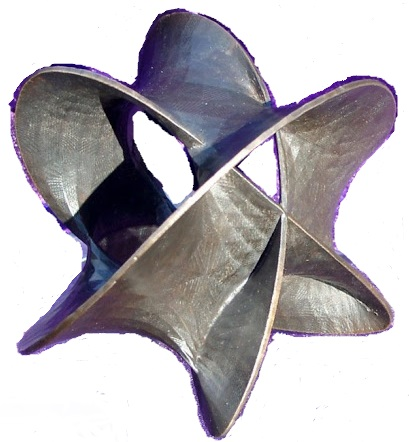
\includegraphics[width=2cm]{K3}};
  \draw[dashed, color=gray] (0,0,0) -- (0,0,4);
    \draw[dashed, color=gray] (0,0,0) -- (0,4,0);
    \draw[dashed, color=gray] (0,0,0) -- (4,0,0);
    \draw (0,4,0) -- (0,0,4);
    \draw (0,4,0) -- (4,0,0);
    \draw (4,0,0) -- (0,0,4);

	\end{tikzpicture}
\end{center}

\begin{comment}
\begin{center}
 \begin{tikzpicture}
   \node[opacity=0.3] (img1) at (0.8453,0.8453,0.8453) {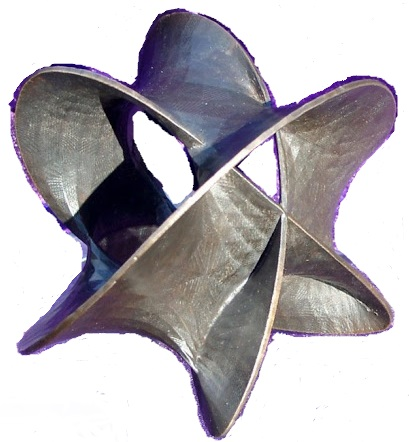
\includegraphics[width=2cm]{K3}};
  \draw[dashed, color=gray] (0,0,0) -- (0,0,4);
    \draw[dashed, color=gray] (0,0,0) -- (0,4,0);
    \draw[dashed, color=gray] (0,0,0) -- (4,0,0);
    \draw (0,4,0) -- (0,0,4);
    \draw (0,4,0) -- (4,0,0);
    \draw (4,0,0) -- (0,0,4);

    \filldraw[gray] (0.8453,0.8453,0) -- (0.8453,0.8453,0.8453) -- (0.8453,0,0.8453) -- (0.8453,0,0) -- cycle;
 %   \draw (0.8453,0.8453,0.8453) -- (0.8453,0,0.8453);

	\end{tikzpicture}
\end{center}
\end{comment}

\subsection{Тропический миррор (анонс)}

В А-модели задача формулируется так: сколько определённых кривых\que{картинка?} пройдёт через отмеченные циклы\que{здесь тонкость: нужно переопределить понятие цикла}.

$$\text{A-сторона:} \hskip 20 pt H = \vec p \cdot \vec n + \sum\limits_{\delta} V_{\delta}$$
$$\text{B-сторона:} \hskip 20 pt H = \frac{\p}{\p \vec x} \frac{\p}{\p \vec y} + e^{\vec \delta \vec y}$$

Видно, что А- и B-стороны связаны просто-напросто Фурье-преобразованием. На B-стороне получается теория поля; так получающаяся теория поля называется теорией Бершадского---Чекотти---Огури---Вафы (только они писали для обычной комплексной структуры, а надо для деформированной суперпотенциалом).

\section{Связь суперконформной теории поля и теории Саито}
\subsection{Строим основной объект, деформируем дифференциал Бельтрами}

Введём несколько пространств модулей:

$$\mathcal{M}_g = \{\text{все дифференциалы Бельтрами}\} / \{\text{диффеоморфизмы}\}$$

$$\mathcal{M}_{g,n} = \{\text{все дифференциалы Бельтрами}\} / \{\text{диффеоморфизмы, обращающиеся в ноль}\}$$

$$\mathcal{\hat M}_{g,n} = \{\text{все дифференциалы Бельтрами}\} / \{\text{диффеоморфизмы, имеющие нулевой росток}\}$$

И объявим главным объектом рассмотрения т.н. <<основной объект>> $I$:

\be I^{(k,l)} = \langle  V_1 (z_1) ... V_n (z_n) \int\limits_{\Sigma} G \cdot \mu^{(1)} ... \int\limits_{\Sigma} G \cdot \mu^{(k)} \int\limits_{\Sigma} \bar G \cdot \bar \mu^{(1)} \int\limits_{\Sigma} \bar G \cdot \bar \mu^{(l)}                          \rangle   \ee

Теперь продеформируем $\mu$ векторным полем: $\mu \to \mu + \bar\p v$ ($v$ не может иметь нули более чем первого порядка, но хотя бы один ноль первого порядка имеет), получим выражение вида $$\int\limits_{\Sigma} \bar\p (Gv)$$
и произведём интегрирование по частям в $\delta I$.


На пространстве вертексных операторов действует $Q_{\varepsilon} = Q + \varepsilon G_0$. Возьмём два каких-то вертексных оператора и потребуем, чтобы $$V_1 - \varepsilon \tilde V_1 = Q_{\varepsilon} (...).$$ Тогда для основного объекта верно $$I(V_1, ...) \sim c_1 (\mathcal{L}_1) \wedge I(\tilde V_1, ...)$$

Подействуем: $$(d + \varepsilon \iota_v) A = F + \varepsilon,$$

$F$ и $\varepsilon$ не просто замкнуты по отдельности, но ещё и их сумма точна. Поэтому $\varepsilon$ представляется первым классом Черна.

Формула Картана и соотношение между тензором энергии-импульса $T$, его суперпартнёром $G$ и дифференциалом де Рама $Q$ невероятно похожи:
$$\mathcal{L}_v  = \{d, \iota_v\}$$
$$T = \{Q, G\}$$

Поэтому эти матфизические величины можно интерпретировать так: $T$ --- то, что представляет диффеоморфизмы, $Q$ --- то, что представляет дифференциал де Рама, $G$ --- то, что представляет подстановку векторного поля.

\subsection{Теория Саито}
Теория Саито отвечает на вопрос <<как построить связность в когомологиях $Q_{\varepsilon}$>>.

Зачем нужна такая связность? Затем, что эта связность наряду со связностью Гаусса---Манина образуют плоский пучок и дают уравнение WDVV.

\subsubsection{Изложение хронологическое}

Сам Саито занимался, как известно, теорией особенностей и начал с изучения таких интегралов: $$\int \frac{\Omega}{W - t_0},$$ а также их производных по $t_0$. Он заметил, что удобно ввести величину $\varepsilon := \Big(\frac{\p}{\p t_0} \Big)^{-1}$. Потом Варченко указал ему, что его интегралы --- то же, что интегралы вида $$\int\limits_{\Gamma} e^{\frac{W}{\varepsilon}} \Omega.$$

Некоторые из них оказываются нулями. При каких условиях?

Рассмотрим самый простой --- одномерный случай, $\Omega = P dx = d\tilde P$. Получаем $$- \int e^{\frac{W}{\varepsilon}} d\tilde P = \int d \Big( e^{\frac{W}{\varepsilon}} \Big) \tilde P = \int \frac{dW}{\varepsilon} e^{\frac{W}{\varepsilon}} \tilde P,$$ $$\int (d + \frac{dW}{\varepsilon}) \tilde P e^{\frac{W}{\varepsilon}} = 0$$ $$\int (\varepsilon d + dW) \tilde P e^{\frac{W}{\varepsilon}} = 0$$

Чтобы искомая связность $\Omega = d\tilde P$ была плоская, надо потребовать $(\varepsilon d + dW) \tilde P = 0$.

Порассматриваем какие-нибудь простейшие суперпотенциалы. Пусть, например, $W = x^2$. Методом неопределённых коэффициентов найдём связность $\tilde P$: $$(\varepsilon d + 2x) (\alpha_0 + \alpha_1 x + \alpha_2 x^2 + \alpha_3 x^3 + ...) = 0$$ $$\Big(\varepsilon \alpha_1 + 2 \varepsilon \alpha_2 x + 3 \varepsilon \alpha_3 x^2 + ...\Big) + \Big(2 \alpha_0 x + 2 \alpha_1 x^2 + 2 \alpha_2 x^3 + ...\Big) = 0,$$ откуда можно вытащить такую череду равенств: $$\varepsilon \alpha_1 = 0$$
$$2 \varepsilon \alpha_2 + 2 \alpha_0 = 0$$
$$3 \varepsilon \alpha_3 + 2 \alpha_1 = 0$$
$$4 \varepsilon \alpha_4 + 2 \alpha_2 = 0$$
 и так далее. Из неё вполне видно, что все нечётные $\alpha_i$ равны нулю, а все чётные удовлетворяют равенству $$\alpha_{2n} = \frac{(-1)^n}{\varepsilon^n n!} \alpha_0.$$ Поэтому плоская связность для такого суперпотенциала равна дифференциалу де Рама от следующего выражения:
 
 $$\tilde P = \alpha_0 - \frac{1}{\varepsilon 1!} \alpha_0 x^2 + \frac{1}{\varepsilon^2 2!} \alpha_0 x^4 + ...$$
 
 Приравняем к единице несущественный общий множитель. Возьмём дифференциал и получим наконец плоскую связность для суперпотенциала $W = x^2$:
 
$$\Omega = d\tilde P = d \sum\limits_n \frac{(-1)^n}{\varepsilon^n n!} x^{2n} = \boxed{\sum\limits_n \frac{(-1)^n}{\varepsilon^n (n-1)!} x^{2n-1} }$$
 
 (множитель $2$ опущен как общий).

Аналогично можно рассмотреть $W = x^3$. 





$\varepsilon$ генерирует $\psi$-классы Мориты---Мамфорда\que{Раскрыть.}.


\subsubsection{Изложение теоретико-полевое}

$$S = \int \Big( \p X \bar \p \bar X + \bar \pi \p \bar \psi + \pi \bar \p \psi  \Big)$$

$$G = \pi \p \bar X$$
$$J = \psi \p X$$

Как устроены поля конформной размерности 0? Вот так: $F(X, \bar X, \psi, \bar \psi)$.

Однако можно сделать замену вида $\rho = \psi + \bar \psi$, $\theta = (\psi - \bar \psi) g$. Тогда внезапно оказывается, что $F(X, \bar X, \rho^{\bar i}, \theta_i)$ --- не что иное, как поливекторные поля со значениями в $(0,\bullet)$-формах.

$$QP = \rho \frac{\p}{\p \bar X} P = \bar \p^{t} P$$

$$G_0 - \bar G_0 = \frac{\p}{\p \theta_i} \frac{\p}{\p X^i} = \Delta_{BV}$$

Это всё было при $W=0$. Если <<включить>> суперпотенциал, ток изменится на такой: $$J = \psi \p X + W' \pi$$ а дифференциал превратится в такой:

$$Q + \varepsilon G_0 = \bar\p + \varepsilon \Delta_{BV} + \frac{\p W}{\p X^i} \frac{\p}{\p \theta_i},$$

$\bar\p$ --- дифференциал свободной теории, $\varepsilon \Delta_{BV}$ --- эквивариантная добавка, $\frac{\p W}{\p X^i} \frac{\p}{\p \theta_i}$ --- вызванное наличием суперпотенциала возмущение.

\section{Топологическая квантовая механика}
\subsection{$A_{\infty}-$структура и один из контекстов её возникновения в матфизике}

Попробуем спасти идею функционального интеграла. Исторически он регуляризовывался введением решётки. Однако, как заметил Колмогоров в 50-е гг.,  на коцепях нет ассоциативного умножения\que{почему?}. На дифференциальных формах есть ассоциативное умножение, а вот на симплициальной реализации того же самого --- как оказалось, нет. Однако там есть почти ассоциативное умножение --- $A_{\infty}$-структура.

Например, $m_2$ ассоциативно с точностью до высших операций:

\begin{center}
 \begin{tikzpicture}

%  \draw[->, color=gray, thick] (0,0) -- (10,0) node[right] {$z_T$};
%  \draw[->, color=gray, thick] (0,0) -- (0,6) node[above] {$w_T$};
  \draw[very thick] (1.5,5) -- (2,4);
    \draw[very thick] (1.5,3) -- (2,4);
    \filldraw [black] (2,4) circle (2pt);
        \filldraw [black] (4,3) circle (2pt);
            \draw[very thick] (2,4) -- (4,3);
            \draw[very thick] (4,3) -- (3.5,2);
            \draw[very thick] (4,3) -- (4.5,2);
  \draw (2,4) node[above=1pt, right=1pt] {$m_2$};
  \draw (4,3) node[above=1pt, right=1pt] {$m_2$};
  
  \draw (1.5,3) node[below=1pt] {$1$};
  \draw (3.5,2) node[below=1pt] {$2$};
  \draw (4.5,2) node[below=1pt] {$3$};
  
    \draw (6,3.5) node {$-$};

  \draw[very thick] (7.5,2) -- (8,3);
    \draw[very thick] (8.5,2) -- (8,3);
    \filldraw [black] (8,3) circle (2pt);
        \filldraw [black] (9,4) circle (2pt);
            \draw[very thick] (8,3) -- (9,4);
            \draw[very thick] (9,4) -- (9.5,3);
            \draw[very thick] (9,4) -- (9.5,5);
  \draw (8,3) node[above=1pt, left=1pt] {$m_2$};
  \draw (9,4) node[above=1pt, left=1pt] {$m_2$};

 \draw (7.5,2) node[below=1pt] {$1$};
  \draw (8.5,2) node[below=1pt] {$2$};
 \draw (9.5,3) node[below=1pt] {$3$};

    \draw (11,3.5) node {$=$};
    
    \draw (12,3.5) node {$d(m_3)$};

	\end{tikzpicture}
\end{center}


Есть $n-$арные операции: элементы $d, m_2, m_3, m_4, ...$. Их можно изобразить так:

\begin{center}
 \begin{tikzpicture}

  
  \draw (0,2.5) -- (0,2) -- (0.5,2) -- (0.5,2.5) -- cycle;
  \draw (-1,2.25) -- (0,2.25);
  \draw (0.5,2.25) -- (1.5,2.25);
    \draw (2,2.25) node[right=1pt] {$d$};
  
    \draw (0,1.5) -- (0,1) -- (0.5,1) -- (0.5,1.5) -- cycle;
  \draw (-1,1.25) -- (0,1.25);
    \draw (-1,1.125) -- (0,1.125);
      \draw (-1,1.375) -- (0,1.375);
  \draw (0.5,1.25) -- (1.5,1.25);
      \draw (2,1.125) node[right=1pt] {$m_3$};

  \draw (0,0.5) -- (0,0) -- (0.5,0) -- (0.5,0.5) -- cycle;
  \draw (-1,0.167) -- (0,0.167);
    \draw (-1,0.33) -- (0,0.33);
  \draw (0.5,0.25) -- (1.5,0.25);
      \draw (2,0.25) node[right=1pt] {$m_2$};

	\end{tikzpicture}
\end{center}

Набор операций $(d, m_2, m_3, ...)$, согласованный с (супер)правилом Лейбница, называется $A_{\infty}$-структурой.

В струнах, конечно, эти диаграммы будут выглядеть как

\begin{center}
\begin{tikzpicture}


%\fill[cyan!10] (4,0) rectangle (0,3);

%\fill[cyan!10] (0.11,3.4) arc (-175:-5:1.9cm and 0.6cm) -- (3.89,2.45) -- (0.11,2.45) -- cycle;
%\fill[cyan!10] (3.89,-0.4) arc (5:175:1.9cm and 0.6cm) -- (0.11,0.55) -- (3.89,0.55) -- cycle;

	\draw[thick] (4,1.5) ellipse (0.166 and 0.5);% right ellipse
	\draw[thick] (0,3) ellipse (0.166 and 0.5);% left top ellipse
	\draw[thick] (0,0) ellipse (0.166 and 0.5);% left bottom ellipse
\draw[thick] (-0.1,0.4) arc (-45:45:1cm and 1.55cm); % left arc
\draw[thick] (4,1) arc (95:178:4.2cm and 1.2cm); % bottom arc
\draw[thick] (0.15,3.2) arc (-180:-95:4.2cm and 1.2cm); % top arc
      \draw (2,-1) node[below=1pt] {$m_2$};

	\draw[thick] (7,1.5) ellipse (0.166 and 0.5);% right ellipse
	\draw[thick] (11,1.5) ellipse (0.166 and 0.5);% left top ellipse
\draw[thick] (7,1) -- (11,1);
\draw[thick] (7,2) -- (11,2);
      \draw (9,-1) node[below=1pt] {$d$ (она же $m_1$)};

\end{tikzpicture}
\end{center}


\subsection{Перенормировки в топологической квантовой механике}

Общепринятым способом избегания УФ расходимостей является введение параметра обрезания:
$$\int d^N p \longrightarrow \int\limits_0^{\Lambda} d^N p$$

Способ ввести параметр обрезания <<в лоб>> в топологической квантовой механике --- ограничиться на формы $\Omega_X^{\bullet \Lambda}$ --- на формы, у которых импульсы, получающиеся после преобразования Фурье функции, стоящей перед $dx^1 \wedge ... \wedge dx^n$, ограничены по модулю числом $\Lambda$: $$\Omega_X^{\bullet \Lambda} := \Omega_X^{\bullet}\Big|_{|\vec p| < \Lambda}, \hskip 20 pt \Omega_X^{\bullet} \longrightarrow \Omega_X^{\bullet \Lambda}.$$ Но на $\Omega_X^{\bullet \Lambda}$ уже нет структуры dg-алгебры\que{кстати, почему?}. Проблема.

Необходим более умный способ перенормировки. (Где здесь вообще может возникнуть расходимость? Она может возникнуть, если вершины сталкиваются. Коррелятор в таком случае может быть не определён, а вклад пропагатора будет стремиться к тождественному оператору.)

Предложение заключается в том, чтобы перейти к швингеровскому представлению пропагатора и затем перенормировать <<время>>:

$$\int\limits_{\tau_{\text{ш}}}^{\infty} d\tau e^{-\tau \Delta} = [\tau' = \tau - \tau_{\text{ш}}] = \int\limits_0^{\infty} d\tau' e^{-(\tau' + \tau_{\text{ш}}) \Delta} = e^{-\tau_{\text{ш}} \Delta} \int\limits_0^{\infty} d\tau' e^{-\tau' \Delta} = e^{-\tau_{\text{ш}} \Delta} \frac{1}{\Delta},$$ т.е. перенормированный пропагатор вот каков:

$$\frac{1}{\Delta_{\text{ren}}} = e^{-\tau_{\text{ш}} \Delta} \frac{1}{\Delta}.$$

Перенормированный таким образом пропагатор будем помечать буквой <<ш>> (швингеровское же представление):

\begin{center}
 \begin{tikzpicture}

\draw (-1,0) -- (1,0);
   \filldraw[color=white, rounded corners] (-0.5,-0.25) rectangle (0.5,0.25);
  \draw[rounded corners] (-0.5,-0.25) rectangle (0.5,0.25);
\node at (0,0) {\text{ш}};

	\end{tikzpicture}
\end{center}

Впоследствии мы будем делать утверждения вида <<такой-то пропагатор чему-то равен>>. В целях удобства обсуждения договоримся опускать в них множитель $1/\Delta$. В рамках этой договорённости у нас получилось, что

\begin{center}
 \begin{tikzpicture}

\draw (-1,0) -- (1,0);
   \filldraw[color=white, rounded corners] (-0.5,-0.25) rectangle (0.5,0.25);
  \draw[rounded corners] (-0.5,-0.25) rectangle (0.5,0.25);
\node at (0,0) {\text{ш}};

    \draw (1.5,0) node {$=$};

    \draw (2.5,0) node {$e^{-\tau_{\text{ш}} \Delta},$};

\draw (3.5,0) -- (5.5,0);
    \draw (6,0) node {$=$};

    \draw (6.5,0) node {$1$};
	\end{tikzpicture}
\end{center}

Пример перенормированной диаграммы:

\begin{center}
 \begin{tikzpicture}



\draw (-1,0) -- (1,0);
%\draw (-0.2,-0.25) -- (-0.2,0.25) -- (0.2,0.25) -- (0.2,-0.25) -- cycle;

\draw (1,0) -- (3,1);
\draw (1,0) -- (3,-1);

\draw (-1,0) -- (-3,1);
\draw (-1,0) -- (-3,-1);

%\tikzset{anchor=west}

\filldraw[color=white, rounded corners] (-0.5,-0.25) rectangle (0.5,0.25);
\draw[rounded corners] (-0.5,-0.25) rectangle (0.5,0.25);
 \draw (0,0) node {\text{ш}};
 
 \filldraw[color=white, rotate around={26.57:(1,0)}, rounded corners] (1.618,-0.25) rectangle (2.618,0.25);
  \draw[rotate around={26.57:(1,0)},rounded corners] (1.618,-0.25) rectangle (2.618,0.25);
  
   \filldraw[color=white, rotate around={-26.57:(1,0)}, rounded corners] (1.618,-0.25) rectangle (2.618,0.25);
  \draw[rotate around={-26.57:(1,0)},rounded corners] (1.618,-0.25) rectangle (2.618,0.25);
  
   \filldraw[color=white, rotate around={26.57:(-1,0)}, rounded corners] (-1.618,-0.25) rectangle (-2.618,0.25);
  \draw[rotate around={26.57:(-1,0)},rounded corners] (-1.618,-0.25) rectangle (-2.618,0.25);
  
   \filldraw[color=white, rotate around={-26.57:(-1,0)}, rounded corners] (-1.618,-0.25) rectangle (-2.618,0.25);
  \draw[rotate around={-26.57:(-1,0)},rounded corners] (-1.618,-0.25) rectangle (-2.618,0.25);
 


%\draw[rotate=0] (2.2,0) node[rotate around={26.57:(1,0)}] {\text{ш}}; 
%\node[rotate around={26.57:(1,0)}] at (2,0.5) {\text{ш}}; 

\node[rotate=26.57] at (2,0.5) {\text{ш}};
\node[rotate=-26.57] at (2,-0.5) {\text{ш}};

\node[rotate=-26.57] at (-2,0.5) {\text{ш}};
\node[rotate=26.57] at (-2,-0.5) {\text{ш}};

%\node[draw, rotate around={60:(-1,0)}]

         
%\foreach \x/\y in {0.8944/0, 1.7889/0, 2.6833/0, 3.5777/0}
 %   \draw[rotate=26.57,dashed,thick,color=cyan] (\x,\y) ellipse (0.1cm and 0.3cm);
 
%\draw[rounded corners,red,rotate around={30:(-1,0.5)}] (-3.5,0) rectangle (-0.5,2);


	\end{tikzpicture}
\end{center}

Дальше мы в шутку будем называть швингеровские пропагаторы резисторами.

Если отнести деформации пропагатора к вершинам и воспринимать их уже как деформации операторов, стоящих в вершинах, то получится как раз $A_{\infty}$-структура.


\subsection{Об аксиальной аномалии}


Далее, есть такой хорошо известный математический факт --- что лапласиан есть суперкоммутатор дифференциала де Рама $d$ и сопряжённого к нему по Ходжу $d^*$. Т.е. $$e^{-\tau_{\text{ш}} \Delta} = e^{-\tau_{\text{ш}} \{ d, d^* \} }$$

Обсудим аномальный распад $\pi^0 \to 2\gamma$.

$$\psi_L \to e^{i\alpha} \psi_L $$

$$\psi_R \to e^{-i\alpha} \psi_R $$

$$\operatorname{Tr}_{\text{Spin}} \gamma^5 e^{-\beta \slashed{D}^2_A} = \operatorname{Str} e^{-\beta \slashed{D}^2_A}$$

Эйлерова характеристика:

$$\chi = \operatorname{Str}_{\Omega^{\bullet}} e^{-\tau_{\text{ш}} \{ d, d^* \}  } $$

Арифметический род:

$$H\chi = \operatorname{Str}_{\Omega^{0,\bullet}} e^{-\tau_{\text{ш}} \{ \bar \p, \bar \p^* \}  } $$

\subsection{Как вычислять амплитуды}

Вот BV-регуляризация по Костелло:

\begin{center}
 \begin{tikzpicture}

\draw (-1,0) -- (1,0);

    \draw (1.5,0) node {=};

    \draw (2.5,0) node {$e^{-\tau_{\text{ш}} \{Q,G\}}$};

   \filldraw[color=white, rounded corners] (-0.5,-0.25) rectangle (0.5,0.25);
  \draw[rounded corners] (-0.5,-0.25) rectangle (0.5,0.25);
\node at (0,0) {\text{ш}};

	\end{tikzpicture}
\end{center}

Рецепт вычисления амплитуд: необходимо проинтегрировать по всем внутренним линиям, а входы и выходы замкнуть на когомологии. Если подстановка резистора (отличие резистора от его отсутствия) --- $Q$-точная вещь:

\begin{center}
 \begin{tikzpicture}
 
\draw (-1,0) -- (1,0);


   \filldraw[color=white, rounded corners] (-0.5,-0.25) rectangle (0.5,0.25);
  \draw[rounded corners] (-0.5,-0.25) rectangle (0.5,0.25);
\node at (0,0) {\text{ш}};

    \draw (1.5,0) node {$-$};
    
        \draw (2,0) node {$1$};

    \draw (2.5,0) node {$=$};

    \draw (3.25,0) node {$Q(..),$};

	\end{tikzpicture}
\end{center}

то ответ не будет зависеть от величины швингеровского обрезания. Нас интересует именно $Q$-точный случай как самый красивый и реалистичный, ибо если на графах существует суперпартнёр тензора энергии-импульса $G$, то подстановка резистора $Q$-точна.


\begin{center}
 \begin{tikzpicture}

\filldraw [black] (0,0) circle (2pt);
\draw (0,0) node[below=1pt] {$0$};

\draw (0,0) -- (1,0);

\filldraw [black] (1,0) circle (2pt);
\draw (1,0) node[below=1pt] {$\tau_{\text{ш}}$};

\draw (3.5,0) node {$= \{Q, \int\limits_0^{\tau_{\text{ш}}} e^{-\tau \{ Q,G\} } G d\tau \}$};


	\end{tikzpicture}
\end{center}

Зачем вводить теорию струн in order to avoid divergences, когда это можно сделать проще с помощью топологической квантовой механики?

\subsection{Постоянная Планка --- скрытое число петель (внутренних и внешних)}

\begin{center}

Фейнман: $e^{\frac{1}{\hbar} S}$

Костелло---Швингер---Цвибах: $e^{\frac{1}{\hbar} S(\hbar)}$

\end{center}

Гений Баталина(?) состоял в том, чтобы написать действие, зависящее от постоянной Планка, а не как у Фейнмана\que{Раскрыть эту мысль и раскрыть мысль, вынесенную в заголовок.}.

Ещё раз: после перехода к дискретному пространству теория струн становится теорией частиц, в которой очень много вершин и пропагаторов между ними. После перехода к дискретному пространству теория струн --- частный случай описанной выше конструкции. Это придумал Цвибах, но побоялся включить в свою книжку по теории струн. 


\bigskip
\bigskip


 \end{document}
